\documentclass[12pt]{report}
\linespread{1.1}
\bibliographystyle{plain}
\usepackage[utf8]{inputenc}
\usepackage{graphicx}
\graphicspath{ {images/} }
\title{Compressive Sensing Chapter}
\author{Thomas Owen Kealy}
\date{\today}

\linespread{1}
\usepackage{wrapfig}
\usepackage{amsfonts}
\usepackage{amsmath}
\usepackage[utf8]{inputenc}
\usepackage[T1]{fontenc}
\usepackage{graphicx}
\usepackage[english]{babel}
\usepackage[algoruled]{algorithm2e}

\renewcommand{\theequation}{\thesection.arabic{equation}}

\renewcommand{\thefigure}{\thesection.\arabic{figure}}



\renewcommand{\vec}[1]{\mathbf{#1}}
\renewcommand{\theequation}{\thesubsection.\arabic{equation}}
\DeclareGraphicsExtensions{.pdf,.png,.jpg, .gif}

\usepackage{amsthm}

\usepackage[english]{babel}
\usepackage{mathtools}

%\usepackage[OT2,T1]{fontenc}
%\DeclareSymbolFont{cyrletters}{OT2}{wncyr}{m}{n}
%\DeclareMathSymbol{\sha}{\mathalpha}{cyrletters}{"58}

\DeclareFontFamily{U}{wncy}{}
\DeclareFontShape{U}{wncy}{m}{n}{<->wncyr10}{}
\DeclareSymbolFont{mcy}{U}{wncy}{m}{n}
\DeclareMathSymbol{\Sh}{\mathord}{mcy}{"58} 
\DeclareMathOperator*{\argmin}{arg\,min}

\newcounter{eqn}
\renewcommand*{\theeqn}{\alph{eqn})}
\newcommand{\num}{\refstepcounter{eqn}\text{\theeqn}\;}

\makeatother
\newcommand{\vectornorm}[1]{\left|\left|#1\right|\right|}
\newcommand*\conjugate[1]{\bar{#1}}


\newtheorem{thm}{Theorem}
\newtheorem{defn}{Definition}
 %\theoremstyle{plain}
  \newtheorem{theorem}{Theorem}[section]
  \newtheorem{corollary}[theorem]{Corollary}
  \newtheorem{proposition}[theorem]{Proposition}
  \newtheorem{lemma}[theorem]{Lemma}
\newtheorem{example}[theorem]{Example}
  \newtheorem{definition}[theorem]{Definition}
  \newtheorem{conj}[theorem]{Conjecture}
 \newtheorem{condition}{Condition}
 \newtheorem{remark}[theorem]{Remark}

\newcommand{\supp}{\operatorname{supp}} 
\newcommand{\vc}[1]{{\mathbf{ #1}}}
\newcommand{\tn}{\widetilde{\nabla}_{n} }
\newcommand{\Z}{{\mathbb{Z}}}
\newcommand{\re}{{\mathbb{R}}}
\newcommand{\II}{{\mathbb{I}}}
\newcommand{\ep}{{\mathbb{E}}}
\newcommand{\pr}{{\mathbb{P}}}
\newcommand{\FF}{{\mathcal{F}}}
\newcommand{\TT}{{\mathcal{T}}}
\newcommand{\phin}{\phig{n}}
\newcommand{\phig}[1]{\phi^{(#1)}}
\newcommand{\ol}[1]{\overline{#1}}
\newcommand{\eff}{{\rm eff}}
\newcommand{\suc}{{\rm suc}}
\newcommand{\tends}{\rightarrow \infty}
\newcommand{\setS}{{\mathcal{S}}}
\newcommand{\setP}{{\mathcal{P}}}
\newcommand{\setX}{{\mathcal{X}}}
\newcommand{\nec}{{\rm nec}}
\newcommand{\bd}{{\rm bd}}

\begin{document}
\maketitle

\tableofcontents

\section{Introduction and Preliminaries}  \label{sec:intro}

Compressive sensing is a modern signal acquisition technique in which randomness is used as an effective sampling strategy. In practice many signals encountered 'in the wild' can be fully specified by much fewer bits than required by the Nyquist sampling theorem. This is either a natural property of the signals, for example images have large areas of similar pixels, or as a conscious design choice, for example training sequences in communication transmissions. These signals are not statistically white, and so these signals may be compressed (to save on storage). For example, lossy image compression algorithms can reduce the size of a stored image to about 1\% of the size required by Nyquist sampling. 

Whilst this vein of research has been extraordinarily successful, it poses the question: if the reconstruction algorithm is able to reconstruct the signal from this compressed representation, why collect all the data in the first place, when most of the information can be thrown away? 

Compressed Sensing answers these questions, by way of providing an alternative signal acquisition method to the Nyquist theorem. Specifically, situations are considered where fewer samples are collected than traditional sensing schemes. That is, in contrast to Nyquist sampling, Compressive Sensing is a method of measuring the informative parts of a signal directly without acquiring unessential information at the same time. 

Signals which are compressible, are signals whose information content is smaller than the ambient dimension they are acquired in. Such signals have representations in which they are sparse (i.e. the most of the co-efficients in that representation are zero, or close to zero). For example, 

\begin{enumerate}
\item  A sine wave at frequency \(\omega\) is defined as a single spike in the frequency domain yet has an infinite support in the time domain
\item An image will have values for every pixel, yet the wavelet decomposition of the image will typically only have a few non-zero coefficients
\end{enumerate} 

Informally, CS posits that for \(s\)-sparse signals \(\in \re^{n}\) - signals with \(s\) non-zero amplitudes at unknown locations) - \(\mathcal{O}(s\log{n})\) measurements are sufficient to exactly reconstruct the signal.

In practice this can be far fewer samples than conventional sampling schemes. For example a megapixel image requires 1,000,000 Nyquist samples, but can be perfectly recovered from 96,000 compressive samples in the wavelet domain \cite{watkincandes}. 

As in classical sensing, the measurements are acquired linearly:

\begin{equation}
y_i = \langle \alpha, \psi_i \rangle
\end{equation}

where, \(y_i\) is the \(i^{th}\) sample, \(\alpha \in \re^n\) is the signal, and \(\psi_i\) is the \(i^{th}\) sensing vector.

We require that sensing vectors satisfy two technical conditions (described in detail below): an Isotropy property, which means that components of the sensing vectors have unit variance and are uncorrelated, and an Incoherence property, which means that sensing vectors are almost orthogonal. Once the set of measurements have been taken, the signal may be reconstructed from a simple linear program.

\subsection{RIP and Stable Embeddings}

A high-dimensional signal is sparse, if most of the coefficients \(x_i\) in the linear expansion 

\begin{equation}
\alpha = \sum	_{i=1}^{n} x_i \phi_i
\end{equation}

are zero, where \(x \in \re^n\), \(\alpha \in \re\), and \(\phi_i\) are a set of basis functions of \(\re^n\). We can make the notion of sparsity precise by defining \(\Sigma_s\) as the set of \(s\)-sparse signals in \(\re^n\):

\begin{definition}
\begin{equation}
\Sigma_s = \{ x \in \re^n : |\mathrm{supp} \left(x\right) |\leq s\}
\end{equation}
where \(\mathrm{supp}\left(x\right) \) is the set of indices on which \(x\) is non-zero.
\end{definition}

\begin{figure*}[h]
\centering
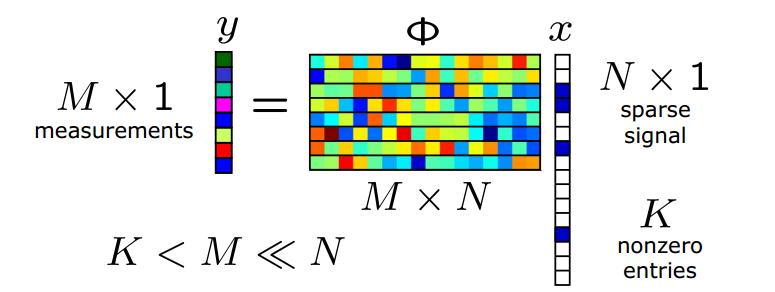
\includegraphics[height = 7 cm, width=\textwidth]{compressive_sensing_example.jpg}
\caption{A visualisation of the Compressive Sensing problem as an under-determined system}
\label{l1l2}
\end{figure*}


We may not be able to directly obtain these coefficients, as we may not posses an appropriate measuring device or one may not exist, or there is considerable uncertainty about where the non-zero coefficients are. Yet we still are able to measure correlations between the signal and some waveforms \(\psi_{k}\) i.e. 

\begin{equation}
y_{k} = \left\langle \alpha \text{,} \psi_{k} \right\rangle \text{ } k = 1 \ldots m
\end{equation}


Given a signal \(\alpha \in \re^n\), a matrix \(A \in \re^{m \times n}\), with \(m \ll n\),  we can acquire the signal via the set of linear measurements:

\begin{equation}
y = Ax
\end{equation}

where in this case \(A\) represents the sampling system (i.e the columns of \(A\) are the products of the two bases \(\psi\), \(\phi\)). In contrast to classical sensing, which requires that \(m = n\) for there to be no loss of information, it is possible to reconstruct \(x\) from an under-determined set of measurements as long as \(x\) is sparse in some basis. 

There are two conditions the matrix \(A\) needs to satisfy for recovery below Nyquist rates:

\begin{enumerate}
\item Restricted Isometry Property.
\item Incoherence between sensing and signal bases.
\end{enumerate}

\begin{definition}[RIP]\label{def:RIP}
We say that a matrix \(A\) satisifes the RIP of order \(s\) if there exists a \(\delta \in \left(0, 1\right)\) such that for all \(x \in \Sigma_s\):

\begin{equation}
\left(1 - \delta\right) \vectornorm{x}_2^2 \leq \vectornorm{Ax}_2^2 \leq \left(1 + \delta\right) \vectornorm{x}_2^2
\end{equation}
i.e. \(A\) approximately preserves the lengths of all \(s\)-sparse vectors in \(\re^n\). 
\label{def:RIP}
\end{definition}

\begin{remark}
Although the matrix \(A\) is not square, the RIP (\ref{def:RIP}) ensures that \(A^TA\) is close to the identity, and so \(A\) behaves approximately as if it were orthogonal. This is formalised in the following lemma from \cite{shalev2014understanding}:

\begin{lemma}
Let A be a matrix which satisfies the RIP of order 2\(s\) with RIP constant \(\delta\). Then for two disjoint subsets \(I, J \subset \left[n\right]\) each of size at most \(s\), and for any vector \(u \in \re^n\):

\begin{equation}
\langle Au_I, Au_J \rangle \leq \delta \vectornorm{u_I}_2^2 \vectornorm{u_J}_2^2
\end{equation}
\\
where \(u_I\) is the vector with component \(u_i\) if \(i \in I\) and zero elsewhere.

\end{lemma}

\end{remark}

\begin{remark} [Information Preservation]
A necessary condition to recover all \(s\)-sparse vectors from the measurements \(Ax\) is that \(Ax_1 \neq Ax_2\) for any pair \( x_ \neq x_2\), \(x_1, x_2 \in \Sigma_s\), which is equivalent to \(\vectornorm{A\left(x_1 - x_2\right)}_2^2 > 0\). 

This is guaranteed as long as \(A\) satisfies the RIP of order 2\(s\) with constant \(\delta\) - as the vector \(x_1 - x_2\) will hve at most \(2s\) non-zero entries, and so will be distinguishable after multiplication with \(A\). To complete the argument take \(x = x_1 - x_2\) in definition \eqref{def:RIP}, guaranteeing \(\vectornorm{A\left(x_1 - x_2\right)}_2^2 > 0 \), and requiring the RIP order of \(A\) to be \(2s\).
\end{remark}

\begin{remark} [Stability]
We also require that the dimensionality reduction of compressed sensing is the preservation of relative distances: that is if \(x_1\) and \(x_2\) are far apart in \(\re^n\) then their projections \(Ax_1\) and \(Ax_2\) are far apart in \(\re^m\). This will guarantee that the dimensionality reduction is robust to noise. 
\end{remark}

A requirement on the matrix \(A\) that satisfies both of these conditions is the following:

\begin{definition}[\(\delta\)-stable embedding]
We say that a mapping is a \(\delta\)-stable embedding of \(U,V \subset \re^n\) if

\begin{equation}
\left(1 - \delta \right) \vectornorm{u-v}_2^2 \leq \vectornorm{Au-Av}_2^2 \leq \left(1 + \delta\right) \vectornorm{u-v}_2^2
\end{equation}

for all \(u \in U\) and \(v \in V\). 
\label{def:d-stable}
\end{definition} 

\begin{remark}
Note that a matrix \(A\), satisfying the RIP of order \(2s\) is a \(\delta\)-stable embedding of \(\Sigma_s, \Sigma_s\). 
\end{remark}

\begin{remark}
Definition \ref{def:d-stable} has a simple interpretation: the matrix \(A\) must approximately preserve Euclidean distances between all points in the signal model \(\Sigma_s\).
\end{remark}

Given that we know a basis in which our signal is sparse, \(\phi\), how do we choose \(\psi\), so that we can accomplish this sensing task? In classical sensing, we choose \(\psi_k\) to be the set of \( T_s \)-spaced delta functions (or equivalently the set of \( 1/T_s \) spaced delta functions in the frequency domain). A simple set of \(\psi_k\) would be to choose a (random) subset of the delta functions above.

In general, we seek waveforms in which the signals' representation would be dense.

\begin{definition}[Incoherence]
A pair of bases is said to be incoherent if the largest projection of two elements between the sensing (\(\psi\)) and representation (\(\phi\)) basis  is in the set \( [1 , \sqrt{n}] \), where \( n \) is the dimension of the signal. The coherence of a set of bases is denoted by \(\mu\).
\end{definition}
Examples of pairs of incoherent bases are:

\begin{itemize}
\item Time and Fourier bases: Let \(\Phi = \textbf{I}_n\) be the canonical basis and \(\Psi = \textbf{F}\) with \(\psi_i = n^{-1\\2}e^{i\omega k} \) be the Fourier basis, then \(\mu\left(\phi, \psi\right) = 1\). This corresponds to the classical sampling strategy in time or space.
\item Consider the basis \(\Phi\) to have only entries in a single row, then the coherence between \(\Phi\) and any fixed basis \(\Psi\) will be \(\sqrt{n}\).
\item Random matrices are incoherent with any fixed basis \(\Psi\). We can choose \(\Phi\) by creating \(n\) orthonormal vectors from \(n\) vectors sampled independently and uniformly on the unit sphere. With high probability \(\mu = \sqrt{n\log{n}}\). This extends to matrices whose rows are created by sampling independent Gaussian or Bernoulli random vectors.
\end{itemize}

This implies that sensing with incoherent systems is good (in the sine wave example above it would be better to sample randomly in the time domain as opposed to the frequency domain), and efficient mechanisms ought to acquire correlations with random waveforms (e.g. white noise).

\textbf{Theorem} \cite{Candes2006}
Fix a signal f \(\in \mathbb{R}^n\) with a sparse coefficient basis, \(x_{i}\) in \(\phi\). Then a reconstruction from \(m\) random measurements in \(\psi\) is possible with probability \(1 - \delta\) if: 

\begin{equation}
m \geq C \mu^2(\phi, \psi) S \log\left(\frac{n}{\delta}\right)
\end{equation}
\label{minsamples}

where \( \mu(\phi, \psi)\) is the coherence of the two bases, and \(S\) is the number of non-zero entries on the support of the signal.

\subsection{Random Matrix Constructions} \label{sec:mtx-contruction}

To construct matrices satisfying definition \ref{def:d-stable}, given \(m, n\) we generate \(A\) by \(A_{ij}\) being i.i.d random variables from distributions with the following conditions \cite{davenport2010signal}

\begin{condition}[Norm preservation]
\(\ep A_{ij}^2 = \frac{1}{m}\)
\label{cond:norm-pres}
\end{condition}

\begin{condition}[sub-Gaussian]
\(\ep\left( e^{A_{ij}t} \right) \leq e^{C^2 t^2 /2}\)
\label{cond:sub-Gauss}
\end{condition}

Random variables \(A_{ij}\) satisfying conditions \eqref{cond:norm-pres} and \eqref{cond:sub-Gauss} satisfy the following concentration inequality \cite{baraniuk2008simple}:

\begin{lemma}[sub-Gaussian]
\begin{equation}
\pr\left( \mid \vectornorm{Ax}_2^2 - \vectornorm{x}_2^2 \mid \geq \varepsilon  \vectornorm{x}_2^2 \right) \leq 2e^{-cM\varepsilon^2}
\label{cond:sub-Gauss concetration}
\end{equation} 
\end{lemma}

Then in \cite{baraniuk2008simple} the following theorem is proved:

\begin{theorem}
Suppose that \(m\), \(n\) and \(0 < \delta < 1\) are given. If the probability distribution generating \(A\) satisfies condition \eqref{cond:sub-Gauss concetration}, then there exist constants \(c_1, c_2\) depending only on \(\delta\) such that the RIP \eqref{def:RIP} holds for \(A\) with the prescribed \(\delta\) and any  \(s \leq \frac{c_1 n}{\log{n/s}}\) with probability \(\geq 1-2e^{-c_2n}\) 
\end{theorem}

For example, if we take \(A_{ij} \sim \mathcal{N}\left(0, 1/m\right)\), then the matrix \(A\) will satisfy the RIP 

\subsection{Wishart Matrices}

Let \(\{X_i\}_{i=1}^r\) be a set of i.i.d \(1 \times p\) random vectors drawn from the multivariate normal distribution with mean 0 and covariance matrix \(H\).

\begin{equation}
X_i = \left(x_1^{(i)}, \ldots , x_p^{(i)}\right) \sim N\left(0, H\right)
\end{equation}

We form the matrix \(X\) by concatenating the \(r\) random vectors into a \(r \times p\) matrix.

\begin{definition}[Wishart Matrix]
Let 

\begin{equation}
W = \sum_{j=1}^r X_j X_j^T =  X X^T
\end{equation}

Then \(W \in \re^{r \times r}\) has the Wishart distribution with parameters 

\begin{equation}
W_r\left(H, p\right)
\end{equation}

where \(p\) is the number of degrees of freedom.
\end{definition}

\begin{remark}
This distribution is a generalisation of the Chi-squared distribution: let \(p = H = 1\). 
\end{remark}

\begin{theorem}[Expected Value]
\begin{equation}
\ep\left(W\right) = rH
\end{equation}
\end{theorem}
\begin{proof}
\begin{align*}
\ep\left(W\right) &= \ep\left(\sum_{j=1}^r X_j X_j^T\right) \\
&= \sum_{j=1}^r \ep\left(X_jX_j^T\right) \\
&= \sum_{j=1}^r \left( \mathrm{Var}(X_j) + \ep(X_j) \ep(X_j^T)   \right) \\
&= rH 
\end{align*}
Where the last line follows as \(X_j\) is drawn from a distribution with zero mean.
\end{proof}

\begin{remark}
The matrix \(M = A^TA\), where \(A\) is constructed by the methods from section \ref{sec:mtx-contruction}, will have a Wishart distribution. In particular, it will have \(\ep M = \frac{1}{m}I_n\) 
\label{remark: exp AtA}
\end{remark}

The joint distribution of the eigenvalues is given by \cite{levequeMatrices}:

\begin{equation}
p\left(\lambda_1, \ldots, \lambda_r\right) = c_r \prod_{i=1}^r e^{-\lambda_i}\prod_{i<j}\left(\lambda_i - \lambda_j\right)^2
\end{equation}

The eigenvectors are uniform on the unit sphere in \(\re^{r}\).

\subsection{Reconstruction Algorithms}
Compressive sensing places the computational load on reconstructing the Nyquist samples \(x\), from the set of compressive samples \(y\). This is in contrast to traditional sensing, where the heavy lifting computationally is done by the process with discretises the continuous signal to create the digital samples. 

Many recovery algorithms have been proposed, and all are based upon minimising some functional of the data. Generally, this is based upon two terms: a data fidelity term, minimising the discrepancy between the reconstruction and the true data, and regularisation term, biasing the reconstruction towards a class of solutions with desirable properties, for example sparsity. Typically the squared error \( \frac{1}{2}\vectornorm{y-Ax}_2^2 \) is chosen as the data fidelity term, whilst a number of regularisation terms have been introduced in the literature. 

A particularly important functional is:

\begin{equation}
\argmin_x \vectornorm{x}_1 \text{ s.t } y=Ax
\label{program:bp}
\end{equation}

known as Basis Pursuit \cite{Chen1998a}, with the following program known as the LASSO \cite{tibshirani1996regression} as a noisy generalisation: 

\begin{equation}
\argmin_x \frac{1}{2}\vectornorm{Ax-y}_2^2 + \lambda\vectornorm{x}_1
\label{program:lasso}
\end{equation}

The statistical properties of LASSO have been well studied. The program performs, both regularisation and variable selection: the parameter \(\lambda\) trades of data fidelity and sparsity with higher values of \(\lambda\) leading to sparser solutions. 

The LASSO shares several features with Ridge regression, and the Non-negative garotte (used for subset regression). It can be shown \cite{hastie2005elements}, that the solution to \eqref{program:lasso} can be written as:

\begin{equation}
\hat{x} = S_{\lambda}\left(x^{OLS}\right) = x^{OLS} \mathrm{sign}\left(x_i - \lambda\right)
\label{soln:lasso}
\end{equation} 

where \(x^{OLS} = (A^TA)^{-1}A^Ty \), whereas the solution to Ridge regression:

\begin{equation}
\argmin_x \frac{1}{2}\vectornorm{Ax-y}_2^2 + \lambda\vectornorm{x}_2^2
\label{program:ridge}
\end{equation}

can be written as:

\begin{equation}
\hat{x} = \left(1+\lambda\right)^{-1}x^{OLS}
\label{soln:ridge}
\end{equation}

and the solution to the best subset regression:

\begin{equation}
\argmin_x \frac{1}{2}\vectornorm{Ax-y}_2^2 + \lambda\vectornorm{x}_0
\label{program:ell0}
\end{equation}

where \( \vectornorm{x}_0 = \{ |i| : x_i \neq 0 \} \), can be written as:

\begin{equation}
\hat{x} = H_{\lambda}\left(x^{OLS}\right) = x^{OLS} \mathbb{I}\left(|x^{OLS}| > \lambda\right)
\label{soln:l0}
\end{equation} 

where \(\mathbb{I}\) is the indicator function. From \eqref{soln:l0} and \eqref{soln:ridge}, we can see that the solution to \eqref{program:lasso}, \eqref{soln:lasso}, translates coefficients towards zero by a constant factor, and set coefficients to zero if they are too small; thus the LASSO is able to perform both model selection (choosing relevant covariates) and regularisation (shrinking model coefficients). 

\begin{figure*}[h]
\centering
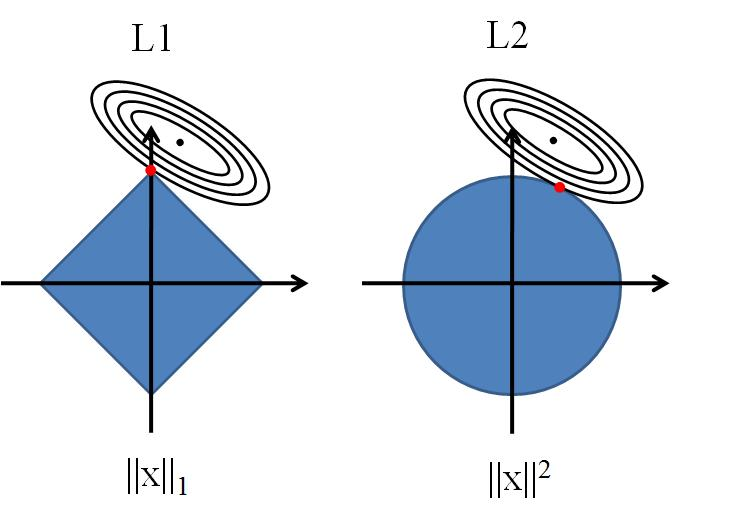
\includegraphics[height = 7 cm]{l1l2.jpg}
\caption{Solutions to the Compressive Sensing optimisation problem intersect the \(l_1\) norm the points where all components (but one) of the vector are zero (i.e. it is sparsity promoting) \cite{Tibshirani1996}}
\label{fig:l1l2}
\end{figure*}

Figure \eqref{fig:l1l2}, provides a graphical demonstration of why the LASSO promotes sparse solutions. \eqref{program:lasso} can also be thought of as the best convex approximation of the \(\ell_0\) problem \eqref{program:ell0}, as the \(\ell_1\)-norm is the convex hull of the points defined by \(\vectornorm{x}_p\) for \(p < 1\) as \(p \rightarrow 0\). 

%The representative algorithm for this type of minimisation is Basis-Pursuit . %

Other examples of regularisers are:

\begin{itemize}
\item Elastic Net: This estimator is a blend of both \eqref{program:lasso} and \eqref{program:lasso}, found by minimising:

\begin{equation}
\argmin_x \frac{1}{2}\vectornorm{Ax-y}_2^2 + \lambda\vectornorm{x}_2^2 + \mu\vectornorm{x}_1
\label{program:enat}
\end{equation}

The estimate has the benefits of both Ridge and Lasso regression: feature selection from the LASSO, and regularisation for numerical stability (useful in the under-determined case we consider here) from Ridge regression. The Elastic-net will outperform the LASSO when there is a high degree of collinearity between coefficients of the true solution.

\item TV regularisation

\begin{equation}
\argmin_x \frac{1}{2}\vectornorm{Ax-y}_2^2 +  \lambda\vectornorm{\nabla x}_1
\label{program:enat}
\end{equation}

This type of regularisation is used when preserving edges whilst simultaneously de-noising a signal is required. It is used extensively in image processing, where signals exhibit large flat patches alongside large discontinuities between groups of pixels.

\item Candes and Tao in \cite{candes2007dantzig}, propose an alternative  functional:

\begin{equation}
\min_{x \in \re^n} \vectornorm{x}_1 \text{ s.t. } \vectornorm{A^T(Ax-y)}_{\infty} \leq t\sigma
\end{equation}

with \(t = c\sqrt{2\log{n}}\). Similarly to the LASSO this functional selects sparse vectors consistent with the data, in the sense that the residual \(r = y - Ax\) is smaller than the maximum amount of noise present. In \cite{candes2007dantzig} it was shown that the \(l_2\) error of the solution is within a factor of \(\log{n}\) of the ideal \(l_2\) error. More recent work by Bikel, Ritov, and Tsybakov, \cite{bickel2009simultaneous}, has shown that the LASSO enjoys similar properties.
\end{itemize}

%Convex algorithms all relax the \(l\)-0 requirement for recovery \cite{tropp2006relax}, by instead solving the equivalent \(l\)-1 minimisation problem:%

Broadly reconstruction algorithms fall into three classes: convex-optimisations/linear programming, greedy methods, and Bayesian methods. Convex optimisation methods offer better performance, measured in terms of reconstruction accuracy, at the cost of greater computational complexity. Greedy methods are relatively simpler, but don't have the reconstruction guarantees of convex algorithms. Bayesian methods offer the best reconstruction guarantees, as well as uncertainty estimates about the quality of reconstruction, but come with considerable computational complexity.

A recent greedy method, Approximate Message Passing (AMP), is a blend of both greedy and Bayesian methods \cite{donoho2009message}.

Convex methods cast the optimisation objective either as a linear program with linear constraints, or as a second order cone program with quadratic constraints. Both of these types of program can be solved with first order interior point methods. However, their practical application to compressive sensing problems is limited due to their polynomial dependence upon the signal dimension and the number of constraints. 

Compressive Sensing poses a few difficulties for convex optimisation based methods. In particular, many of the unconstrained objectives are non-smooth meaning methods based upon descent down a smooth gradient are inapplicable. 

To overcome these difficulties, a series of algorithms originally proposed for wavelet-based image de-noising have been applied to CS, known as iterative shrinkage methods. These have the desirable property that they boil down to matrix-vector multiplications and component-wise thresholding.

Iterative shrinkage algorithms replace searching for a minimal facet of a complex polytope by a iteratively denoised gradient descent. The choice of the (component-wise) denoiser is dependent upon the regulaiser used in \ref{program:lasso}. These algorithms have an interpretation as Expectation-Maximisation \cite{figueiredo2003algorithm} - where the E-step is performed as gradient descent, and the M-step is the application of the denoiser.

\begin{figure}
\begin{algorithmic}[1]
\Procedure{IST}{$y,A, \mu, \tau, \varepsilon$}
\State $x^0 = 0$
\While{$\vectornorm{x^{t} - x^{t-1}}_2^2 \leq \varepsilon$}
\State $x^{t+1} \gets S_{\mu\tau}\left(x^t + \tau A^Tz^t \right) $
\State $z^t \gets y - Ax^t$
\EndWhile
\State \textbf{return} $x^{t+1}$
\EndProcedure
\end{algorithmic}
\caption{The Iterative Soft Thresholding Algorithm}\label{alg:IST}
\end{figure}

%There has been a line of work on algorithms directly minimising the \(l\)-0 norm \cite{wen2015efficient}, \cite{oxvig2012improving}, \cite{mohimani2010sparse}.

Greedy methods are another family of solutions to \ref{program:lasso}. They offer reduced computational complexity with correspondingly worse reconstruction quality and poorer guarantees on sparsity and undersampling than convex algorithms. Examples of this type are Orthogonal Matching Pursuit (OMP)\cite{tropp2007signal}, and Compressive Sensing Orthogonal Matching Pursuit (CoSAMP). 


\begin{figure}
\begin{algorithmic}[1]
\Procedure{OMP}{$y,A,K,\varepsilon$}
\State $x^0 = 0$, $r=y$, $\Omega = \varnothing$, $i=0$
\While{$\vectornorm{x^{t} - x^{t-1}}_2^2 \leq \varepsilon$}
\State $i \gets i+1$
\State $b\gets A^Tr$
\State $\Omega \gets \Omega \cup \mathrm{supp}\left(H_1\left(b\right)\right)$
\State $x\restriction_{\Omega} \gets A^T\restriction_{\Omega}x$
\State $x\restriction_{\Omega^c} \gets 0$
\State $b \gets y - Ax$
\EndWhile
\State \textbf{return} $x$
\EndProcedure
\end{algorithmic}
\caption{The OMP recovery algorithm}\label{alg:omp}
\end{figure}

The Greedy family of algorithms abandons exhaustive searches of the solution space in favour of locally optimal single term updates. They proceed by approximating the solution by some active set of columns from the sensinng matrix \(A\) and solving a restricted least-squares problem at each (in the case of OMP). This guarantees a maximal reduction in \(l\)-2 error in each iteration.

Despite their computational simplicity, greedy algorithms have several drawbacks. Primarily they do not come with stable recovery guarantees, and they require a larger number of samples to recover the signal when compared to Bayesian and Convex recovery algorithms. Also, due to their greedy nature, these algorithms are not guaranteed to converge: in fact it can be shown that there exist \(k\)-sparse vectors and sensing matrices \(A\) such that OMP fails to converge in k iterations \cite{wen2013improved}.



\begin{figure}
\begin{algorithmic}[1]
\Procedure{AMP}{$y,A,\varepsilon$}
\State $x^0 = 0$, $z^0=A^Ty$
\While{$\vectornorm{x^{t} - x^{t-1}}_2^2 \leq \varepsilon$}
\State $x^{t+1} \gets S_{\mu\tau}\left(x^t - \tau+ A^Tz^t\right) $
\State $z^{t+1} \gets y - Ax^t + \frac{\vectornorm{x}_0}{m}z^t$
\EndWhile
\State \textbf{return} $x^{t+1}$
\EndProcedure
\end{algorithmic}
\caption{The AMP recovery algorithm}\label{alg:amp}
\end{figure}



Bayesian methods reformulate the optimisation problem into an inference problem. These methods come with a unified theory, and standard methods to produce solutions. The theory is able to handle hyper-parameters in a unified way, provides a flexible modelling framework, and is able to provide desirable statistical quantities such as the uncertainty inherent in the prediction.

Based on the discussion above we can represent the compressive sensing measurements as: 

\begin{equation}
y = Ax
\end{equation}

where \(A\) is a \(K \times	N\) matrix which is the product of the measurement and sparse bases described earlier.

Note that the measurements may be noisy, with the measurement noise represented by a zero mean Gaussian distribution and unknown variance \( \sigma^2 \):

\begin{equation}
y = Ax + n
\end{equation}
\label{CSequation}

Where \textbf{n} is the vector representing the vector of noise, and has the same support as the measurements. 

Previous sections have shown how the weights \(x\) may be found through optimisation methods such as basis pursuit or greedy algorithms. Here, an alternative Bayesian model is described.

From \ref{CSequation} we have a Gaussian likelihood model: 

\begin{equation}
p \left(y \mid z\text{,} \sigma^2 \right) = (2 \pi \sigma^2)^{-K/2} \exp{\left(- \frac{1}{2 \sigma^2} \|y - Ax|_{2}^{2} \right)} 
\end{equation}

The above has converted the CS problem of inverting sparse weight \textbf{w} into a linear regression problem with a constraint (prior) that \textbf{w} is sparse. 

To seek the full posterior distribution over \textbf{w} and \( \sigma^2 \), we can chose a sparsity promoting prior. A popular sparseness prior is the Laplace density functions:

\begin{equation}
p\left(x\mid\lambda\right) = \left(\frac{\lambda}{2}\right)^N exp{-\lambda \sum_{i=1}^{N} |x_i|}
\end{equation}

Note that the solution the convex optimisation problem \ref{program0} corresponds to a maximum \textit{a posteriori} estimate for \(w\) using this prior. I.e this prior is equivalent to using the \(l_1\) norm as an optimisation function (see figure \ref{laplacenormal} \cite{Tibshirani1996}).

\begin{figure*}[h]
\centering
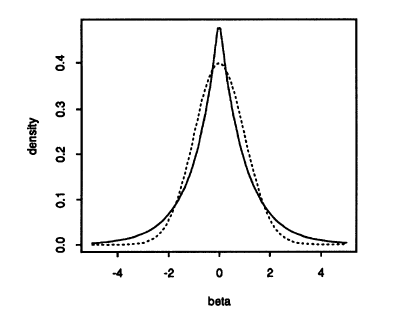
\includegraphics[height = 7 cm]{LaplaceandNormalDensity.png}
\caption{The Laplace (\(l_1\)-norm, bold line) and Normal (\(l_2\)-norm, dotted line) densities. Note that the Laplace density is sparsity promoting as it penalises solutions away from zero more than the Gaussian density. \cite{Tibshirani1996}}
\label{laplacenormal}
\end{figure*}

The full posterior distribution on \(w\) and \(\sigma^2\) may be realised, by using a hierarchical prior instead. To do this, define a zero-mean Gaussian prior on each element of \(w\):
%
\begin{equation}
p\left(w\mid a\right) = \prod_{i=1}^{N}\mathbb{N}\left(w_i\mid 0, \alpha_{i}^-1\right)
\end{equation}
%
where \(\alpha\) is the precision of the distribution. A gamma prior is then imposed on \(\alpha\):

\begin{equation}
p\left(\alpha \mid a, b \right) = \prod_{i=1}^{N} \Gamma\left( \alpha_i \mid a, b \right)
\end{equation}

The overall prior is found by marginalising over the hyperparameters:

\begin{equation}
p\left( w \mid a, b \right) = \prod_{i=1}^{N} \int_{0}^{\infty} \mathbb{N}\left(w_i\mid 0, \alpha_{i}^-1\right) \Gamma\left( \alpha_i \mid a, b \right)
\end{equation}

This integral can be done analytically and is a Student-t distribution. Choosing the parameters \(a,b\) appropriately we can make the Student-t distribution peak strongly around \(w_i = 0\) i.e. sparsifying. This process can be repeated for the noise variance \(\sigma^2\). The hierarchical model for this process is shown in \ref{bayesiancs}. This model, and other CS models which not necessarily have closed form solutions, can be solved via belief-propagation \cite{Baron2010}, or via Monte-Carlo methods.

\begin{figure*}[h]
\centering
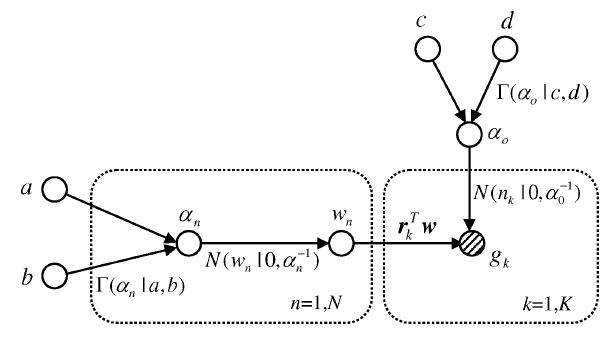
\includegraphics[height = 7 cm]{bayesiancs.png}
\caption{The hierarchical model for the Bayesian CS formulation \cite{Ji2008}}
\label{bayesiancs}
\end{figure*}

However, as with all methodologies, Bayesian algorithms have their drawbacks. Most notable is the use of the most computationally complex recovery algorithms. In particular MCMC methods suffer in high dimensional settings, such as those considered in compressive sensing. There has been an active line of work to address this: most notably Hamiltonian Monte Carlo - an MCMC sampling method designed to follow the typical set of the posterior density. 

Belief propagation (BP) \cite{Yedidia2011} is a popular iterative algorithm, offering improved reconstruction quality and undersampling performance. However, it is a computationally complex algorithm. It is also difficult to implement. Approximate message passing \eqref{alg:amp} solves this issue by blending BP and (IT).

The algorithm proceeds like iterative thresholding, but computes an adjusted residual at each stage. The extra term comes from a first order approximation to the messages passed by BP \cite{metzler2014denoising}.

The choice of prior is key in Bayesian inference, as it encodes all knowledge about the problem. Penalising the least-squares estimate  with the \(\ell_1\) norm, has a Bayesian interpretation as a Laplace distribution prior. This is distinct from the LASSO however, as this Bayesian model does not set coefficients to zero exactly - instead it sets many coefficients to be small. Other priors have been suggested in the literature, such as the Horseshoe  prior, which do set covariates to zero. These do not have the desirable property of leading to closed form posteriors (as shown above).

\section{Compressive Sensing Architechtures}\label{sec:sensingmodel}

\subsection{Modulated Wideband Converter}
We consider a radio environment with a single primary user (PU) and a network of \(J\) nodes collaboratively trying to sense and reconstruct the PU signal, either in a fully distributed manner (by local communication), or by transmitting measurements to a fusion centre which then solves the linear system. 

We try to sense and reconstruct a wideband signal, divided into \(L\) channels. We have a (connected) network of \(J\) (= 50) nodes placed uniformly at random within the square \(  \left[0,1\right]\times \left[0,1\right] \). This is the same model, as in \cite{Zhang2011b}. The calculations which follow are taken from \cite{Zhang2011b} as well.

The nodes individually take measurements (as in \cite{mishali2010theory}) by mixing the incoming analogue signal \(x\left(t\right)\) with a mixing function \(p_i\left(t\right)\) aliasing the spectrum. \(x\left(t\right)\) is assumed to be bandlimited and composed of up to \(k\) uncorrelated transmissions over the \(L\) possible narrowband channels - i.e. the signal is \(k\)-sparse. 

\begin{figure}[h]
\centering
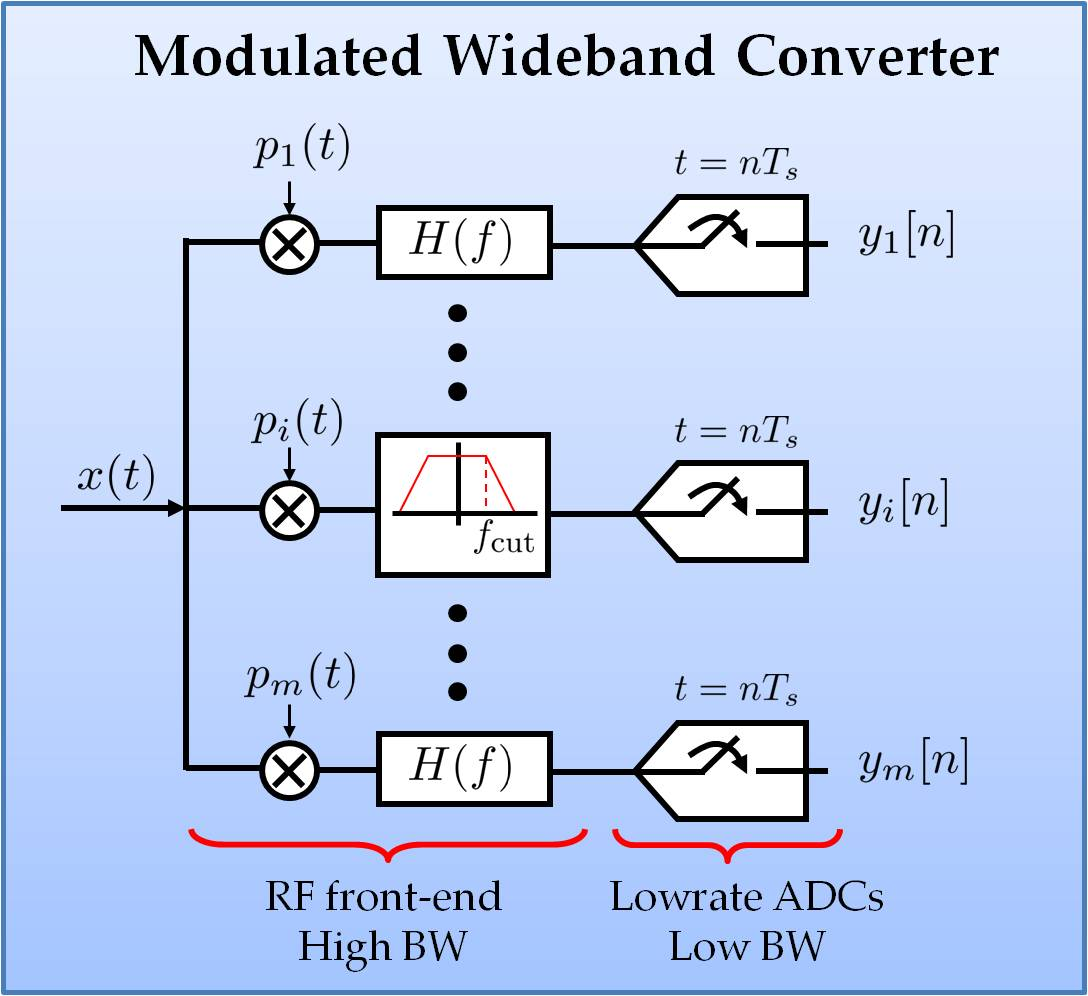
\includegraphics[height = 7.3 cm]{Modulated_wideband_converter.jpg}
\caption{Mse vs SNR for the sensing model, with AWGN only, showing the performance of distributed and centralised solvers}
\label{msevssnr0}
\end{figure}

The mixing functions - which are independent for each node - are required to be periodic, with period \(T_p\). Since \(p_i\) is periodic it has Fourier expansion:

\begin{equation}
p_i\left(t\right) = \sum_{l=-\infty}^{\infty} c_{il} \exp\left({jlt\frac{2\pi}{T_p}}\right)
\end{equation}

The \(c_{il}\) are the Fourier coefficients of the expansion and are defined in the standard manner. The result of the mixing procedure in channel \(i\) is therefore the product \(xp_i\), with Fourier transform (we denote the Fourier Transform of \(x\) by \(X\left( \dot{.} \right)\)):

\begin{align}
X_{i}\left(f\right) &=& \int_{-\infty}^{\infty} x\left(t\right) p_i\left(t\right) dt \nonumber
\\ &=& \sum_{l=-\infty}^{\infty} c_{il} X\left(f-lf_p\right)
\end{align}

(We insert the Fourier series for \(p_i\), then exchange the sum and integral). The output of this mixing process then, is a linear combination of shifted copies of \(X\left(f\right)\), with at most \(\lceil f_NYQ/f_p\rceil\) terms since \(X\left(f\right)\) is zero outside its support (we have assumed this Nyquist frequency exists, even though we never sample at that rate).

This process is repeated in parallel at each node so that each band in \(x\) appears in baseband.

Once the mixing process has been completed the signal in each channel is low-pass filtered and sampled at a rate \(f_s \geq f_p\). In the frequency domain this is a ideal rectangle function, so the output of a single channel is:

\begin{equation}
Y_i\left(e^{j 2 \pi f T_s }\right) = \sum_{l = -L_0}^{+L_0} c_{il} X\left(f-lf_p\right)
\end{equation}

since frequencies outside of \([-f_s/2, f_s/2]\) will filtered out. \(L_0\) is the smallest integer number of non-zero contributions in \(X\left(f\right)\) over \([-f_s/2, f_s/2]\) - at most \(\lceil f_NYQ/f_p\rceil\) if we choose \(f_s = f_p\). These relations can be written in matrix form as:

\begin{equation}
\textbf{y} = \textbf{A}\textbf{x} + \vec{w}
\label{system}
\end{equation}

where \(\textbf{y}\) contains the output of the measurement process, and \(\textbf{A}\) is a product matrix of the mixing functions, their Fourier coefficients, a partial Fourier Matrix, and a matrix of channel coefficients. \(\textbf{x}\) is the vector of unknown samples of \(x\left(t\right)\). 

i.e. \(\textbf{A}\) can be written: 

\begin{equation}
\textbf{A}^{m\times L} = \textbf{S}^{m\times L} \textbf{F}^{L\times L} \textbf{D}^{L \times L} \textbf{H}^{L \times L}
\end{equation}

The system  \ref{system} can then be solved (in the sense of finding the sparse vector \(\vec{x}\) by convex optimisation via minimising the objective function:

\begin{equation}
\frac{1}{2}\|\textbf{Ax}-\textbf{y}\|_2^2 + \lambda \|\textbf{x}\|_1
\end{equation}

where \(\lambda\) is a parameter chosen to promote sparsity. Larger \(\lambda\) means sparser \(\vec{x}\).

\subsection{Random Demodulator}
We assume that the analogue signal \(x\left(t\right)\) is comprised of a finite number of components from some arbitrary dictionary \(\psi_n\left(t\right)\):

\begin{equation}
x\left(t\right) = \sum_{n=1}^N \alpha_n \psi_n\left(t\right)
\end{equation}

The signal is said to be sparse when there are only a few non-zero \(\alpha_n\). The dictionary elements \(\psi_n\) may have a relatively high bandwidth, but the signal itself will have only a few degrees of freedom.

The signal acquisition method proposed consists of three stages (all analogue processing): demodulation, filtering and uniform sampling. 

Initially, the signal is modulated by a pseudo-random sequence \(p_c\left(t\right)\), which alternates at frequencies at (or above) the Nyquist frequency of \(x\left(t\right)\). The signal is then filtered, through a filter with impulse response \(h\left(t\right)\), before being sampled at rate \(\mathcal{M}\) with a traditional ADC.

The output of this system, \(y\left[m\right]\), can be related to the input \(x\left(t\right)\) via a linear transformation of the coefficient vector \(\alpha_n\). 

To find the transformation \(A\), first consider the output of \(y\left[m\right]\), which is the result of convolution and demodulation followed by sampling at rate \(\mathcal{M}\):

\begin{equation}
y\left[m\right] = \int_{-\infty}^{\infty} x\left(\tau\right)p_c\left(\tau\right)h\left(t - \tau\right)\mid_{t = m\mathcal{M}}d\tau
\end{equation}

and by expanding \(x\left(t\right) = \sum_{n=1}^N \alpha_n \psi_n\left(t\right)\):

\begin{equation}
y\left[m\right] =  \sum_{n=1}^N \alpha_n \int_{-\infty}^{\infty} \psi_n\left(t\right)p_c\left(\tau\right)h\left(m\mathcal{M} - \tau\right)d\tau
\end{equation}

we see that the output can be written as:

\begin{equation}
y = Ax
\end{equation}

with

\begin{equation}
A_{m,n} = \int_{-\infty}^{\infty} \psi_n\left(t\right)p_c\left(\tau\right)h\left(m\mathcal{M} - \tau\right)d\tau
\end{equation}

\bibliography{thesis}

\end{document}